Il formato \textbf{PDF} è la codifica più diffusa per l'archiviazione e condivisione di documenti digitali. L'estrazione di informazioni da file PDF è essenziale per numerose attività di indicizzazione, recupero di dati e analisi del contenuto. Nonostante il \textbf{Portable Document Format} prediliga un layout visivo di un documento, affinché sia garantito un aspetto coerente su qualsiasi piattaforma software e hardware, include una piccola percentuale di elementi strutturali, i quali rendono la fase di estrapolazione di dati piuttosto complessa e difficile \cite{2023arXiv230309957M}. \vspace{7pt} \\
Nel corso degli anni, sin dall'introduzione del formato, sono state sviluppate diverse soluzioni dedite all'estrazione dei dati, evolvendosi di pari passo al progresso tecnologico: dagli algoritmi rules-based, al machine learning, fino a soluzioni legate a modelli di deep learning. Una fra di esse, la quale ha dimostrato in differenti circostanze ottimi risultati, è la libreria \textbf{GROBID}. \vspace{7pt} \\
GROBID è uno strumento progettato per ricavare informazioni da file PDF di origine accademica, riorganizzandoli in un formato strutturato noto come \textbf{XML/TEI}. \vspace{7pt} \\ 
La conversione della risorsa avviene mediante l'impiego di una sequenza di algoritmi di machine learning, adottando un \textbf{approccio modulare} che tenta di adattarsi alle caratteristiche gerarchiche del documento. Inizialmente sono individuate le macro-aree che contraddistinguono la risorsa, come l'introduzione, i capitoli oppure i paragrafi, per poi estrarne il contenuto. \vspace{7pt} \\ 
Ad ogni iterazione viene attivato un determinato modello di apprendimento automatico, al quale viene assegnato un numero limitato di etichette da associare alle sezioni del file. In questo modo è garantita una chiara separazione dei ruoli e delle funzioni, semplificando l'integrazione di risultati generati da ulteriori algoritmi di machine learning. Pertanto, ogni classificazione confluisce nella fase successiva di etichettatura, definendo un percorso a cascata che porta ad un risultato altamente dettagliato \cite{grobid2024}. \vspace{7pt} \\ 
I modelli di machine learning utilizzati dalla libreria si suddividono in due categorie, quali:
\begin{itemize}
    \renewcommand{\labelitemi}{-}
    \item \textbf{Modelli per riga}. \\
    I modelli della prima tipologia operano per ogni riga che compongano il documento, tendenzialmente impiegati qualora debbano essere definite le sezioni principali della risorsa, assicurando un'elevata velocità di computazione a discapito della qualità della classificazione.
    \item \textbf{Modelli per token}. \\
    I modelli per token estraggono le informazioni che effettivamente contiene il documento. Contrariamente ai modelli precedenti, garantisce un'elevata precisione ma richiede tempi di esecuzione superiori.
\end{itemize}
L'immagine \ref{fig:2.2.2-2.1} rappresenta visivamente l'approccio modulare descritto prima. Ogni singola entità contiene al suo interno una combinazione di algoritmi di \textbf{classificazione} e di \textbf{tokenizzazione}, affinché sia acquisita la porzione di contenuto desiderata. La radice raffigura il \textbf{segmentation model} incaricato di stabilire le sezioni usuali di un articolo scientifico, destinate ai modelli successivi che si occuperanno di ricavarne le informazioni.
\begin{figure}[H]
    \centering
    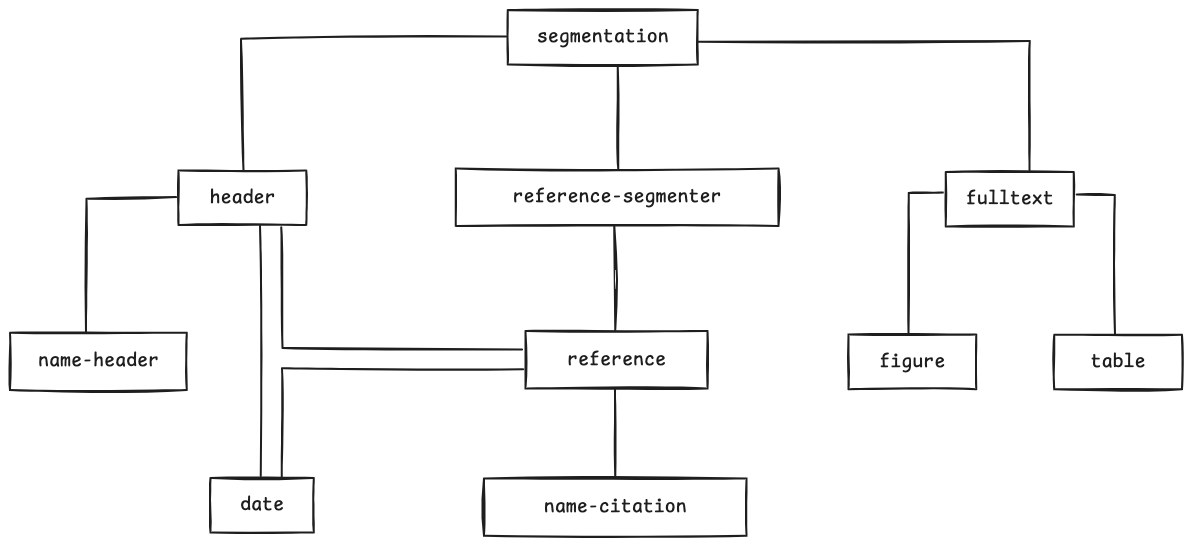
\includegraphics[width=.9\linewidth]{img/img2.png}
    \caption{Raffigurazione dell'approccio modulare di GROBID}
    \label{fig:2.2.2-2.1}
\end{figure} 